For each non-fixed and non-defined variable a propagation queue is made. A propagation queue $q_i$ is an topological 
sort of invariants that are reachable from the vertex representing $x_i$ in $G$ \boste{maybe define topo sort}. The 
propagation queue is used such that each invariant updated at most once if a variable changes value. The DDG show which 
invariant that are directly affected by a change in variable $x_i$ but not the order in which they should be updated. 
The following example show the necessity of such an ordering. 
\begin{center}
    \begin{tikzpicture}[scale=1]
        \vertex[label=$x_1$](x1) at (0,2) {};
        \vertex[label=$i_2$](i2) at (2,1) {};
        \vertex[label=$i_1$](i1) at (4,2) {};
        %\vertex[label=$i_3$](i3) at (5,1) {};
         %\vertex[label=$c_2$](c2) at (5,0) {};
    \tikzset{EdgeStyle/.style={->}}
        \Edge(x1)(i1)
        \Edge(x1)(i2)
        \Edge(i2)(i1)
        %\Edge(x1)(c3)
        %\Edge(y1)(c3)
        %\Edge(y2)(c3)
    \end{tikzpicture}
\end{center}
If $i_1$ is updated before $i_2$ then it might need to be updated again after $i_2$ is updated hence visited twice. In 
worst case this could lead to a exponential number of updates instead of linear. \\ 
Propagation 